\chapter{Introduction to the SSFM for vortex simulations}
\label{ch:splitop}
The Split-Step Fourier Method (SSFM) is an essential technique for simulating a variety of physical systems and is particularly useful for simulating the propagation of wave packets in single and multimode fibers~\cite{agrawal2000, sinkin2003, meirelles2005, min2003} and in various quantum systems~\cite{bayindir2015, weideman1986, wang2005}.
Though other methods, such as explicit and implicit Euler~\cite{butcher2016}, Crank-Nicholson~\cite{crank1947}, and Runge-Kutta~\cite{butcher2016}, can solve similar differential equations, the SSFM has distinct advantages over these methods.
For example, the SSFM is often much easier to parallelize than Runge-Kutta~\cite{brehler2017}, as it primarily relies on embarrassingly parallel element-wise matrix multiplications and Fast Fourier Transform (FFT) routines that have been optimized for parallel and distributed systems.
The SSFM also provides a lower error bound than either the Euler or Crank-Nicholson methods, and does not require an implicit or tridiagonal solver \cite{conte2017, thomas1949} which are also not easily parallelizable~\cite{goddeke2010, wang1981, sweet1977}.
Though much of this work focuses on using the SSFM to simulate superfluid vortex states, I will not be discussing alternative methods, such as vortex-point or vortex-filament simulations in rigorous detail, as this work focuses primarily on engineering appropriate quantum states, while vortex-point and vortex filament methods focus primarily on vortex structures, themselves.

In the work presented here, I will be focusing on the application of the SSFM to superfluid vortex simulations and will use primarily physical arguments to understand the details of the method itself.
I will also discuss several numerical techniques for optimally simulating quantum systems on massively parallel Graphics Processing Units (GPUs), along with software developed for this purpose: GPUE, the Graphics Processing Unit Gross-Pitaevskii Equation Solver.
More details about General Purpose computing with Graphics Processing Units (GPGPU) and the GPUE simulation software can be found in Chapter~\ref{ch:gpu}.
There, I will discuss several additional areas of interest for implementing similar solvers on GPUs, including distributed transposes and important considerations for traditional FFT routines for simulating quantum systems on multiple GPU devices.

This chapter will assume familiarity with basic principles of quantum mechanics and focus on specific performance considerations for simulating quantum systems with the SSFM.
As such, I will also introduce important physical insights for understanding ultracold atomic systems.
In particular, I will focus on understanding superfluid systems created by Bose--Einstein condensation and methods by which we can generate and control vortex dynamics in a Bose--Einstein Condensate (BEC).


\section{The SSFM}
Let us begin with the one-dimensional Schr\"odinger equation,

\begin{equation}
i\hbar \frac{\partial \Psi(r, t)}{\partial t} = \left(\frac{p^2}{2m} + V_0(\mathbf{r}) \right)\Psi(\mathbf{r},t)
\label{eqn:schrody}
\end{equation}

\noindent where $\hat p = -i\hbar\frac{\partial}{\partial x}$ is the canonical momentum operator, $m$ is the mass, $V_0(\mathbf{r})$ is the trapping potential, and $\Psi(r,t)$ is the single-particle wavefunction.
In this case, we often replace most of the right-hand side of the equation with a Hamiltonian operator, which for this case would be $\mathcal{\hat H} = \frac{p^2}{2m} + V_0(\mathbf{r})$.
This noticeably has two components, one acting in position-space, $\mathcal{\hat H}_v = V_0(\mathbf{r})$ and another in momentum-space, $\mathcal{\hat H}_p = \frac{\hat p^2}{2m}$.
For consistency, I will denote all variables in momentum-space with a $p$, and real-space with a $v$.
Additionally, the wavefunction can be expanded into a complete set of eigenkets of the Hamiltonian, with $\mathcal{\hat H}\ket{\Psi_n} = E_n\ket{\Psi_n}$.
One can then write

\begin{equation}
\ket{\Psi(\mathbf{r})} = \sum_{n=0}^N c_n e^{-iE_nt}\ket{\psi_n(\mathbf{r})},
\end{equation}

\noindent where $N$ is the total number of states in the system, $c_n$ is a constant for each constituent eigenfunction $\psi_n(\mathbf{r})$.

Simply stated, the SSFM splits the Hamiltonian into separate operators and uses a Fourier transform on the wavefunction to ensure that these operators are applied in the natural space.
In order to apply the Hamiltonian to the system, we first use a formal solution to the Schr\"odinger equation,

\begin{equation}
\Psi(\mathbf{r},t + dt) = \left[e^{-\frac{i\mathcal{\hat{H}}dt}{\hbar}}\right]\Psi(\mathbf{r},t) = \left[e^{-\frac{i(\mathcal{\hat{H}}_v + \mathcal{\hat{H}}_p)dt}{\hbar}}\right]\Psi(\mathbf{r},t),
\end{equation}

\noindent where $dt$ is a small timestep.
If we assume we are simulating our system by a series of small timesteps, we can split this operation by using the Baker-Campbell-Hausdorff formula,

\begin{equation}
\Psi(\mathbf{r},t+dt) = \left[e^{-\frac{i\mathcal{\hat{H}}_vdt}{\hbar}}e^{-\frac{i\mathcal{\hat{H}}_pdt}{\hbar}}e^{-\frac{[i\hat{H}_v, i\hat{H}_p]dt^2}{2}}\right]\Psi(\mathbf{r},t).
\label{eqn:rsolve}
\end{equation}

\noindent If neglected, the commutation of the real and momentum-space components of the Hamiltonian will accrue an error on the order of $dt^2$.
This is a noticeably high;
however, we can decrease the $dt^2$ error to $dt^3$ by performing a half-step in position space before doing a full-step in momentum space, through a process called Strang splitting~\cite{strang1968},

\begin{equation}
\Psi(\mathbf{r},t+dt) = \left[e^{-\frac{i\mathcal{\hat{H}}_vdt}{2\hbar}}e^{-\frac{i\mathcal{\hat{H}}_pdt}{\hbar}}e^{-\frac{i\mathcal{\hat{H}}_vdt}{2\hbar}} \right]\Psi(\mathbf{r},t) + \mathcal{O}(dt^3).
\end{equation}

Strang splitting can be best understood by performing a Taylor series expansion on both $e^{h(\mathbf{A}+\mathbf{B})}$ and $e^{h\mathbf{A}}e^{h\mathbf{B}}$, where $\mathbf{A}$ and $\mathbf{B}$ are matrices and $h$ is a defined step size~\cite{macnamara2016}.
When expanded,
\begin{equation}
e^{h(A+B)} \approx \mathbf{I} + h(\mathbf{A} + \mathbf{B}) + \frac{1}{2}h^2(\mathbf{A} + \mathbf{B})^2.
\end{equation}

\noindent where $\mathbf{I}$ is the identity matrix.
To the second order terms, the expansion is identical to the expansion of $e^{h\mathbf{A}}e^{h\mathbf{B}}$; however, when expanding the last term, we find,
\begin{equation}
\frac{1}{2}h^2(\mathbf{A} + \mathbf{B})^2 = \frac{1}{2}\left( \mathbf{A}^2 + \mathbf{AB} + \mathbf{BA} + \mathbf{B}^2\right).
\end{equation}

\noindent Here, the $\mathbf{BA}$ term with the expansion of $e^{h\mathbf{A}}e^{h\mathbf{B}}$ because $\mathbf{A}$ always comes before $\mathbf{B}$.
If a symmetric splitting is used instead, it is clear that all the terms up to the second order are the same, such that $e^{h(\mathbf{A}+\mathbf{B})} \approx e^{h\mathbf{A}/2}e^{h\mathbf{B}}e^{h\mathbf{A}/2}$.

Because position and momentum are conjugate domains, after Strang splitting we address each part of this solution in chunks, first in position space, then in momentum space, then in position space again by using Fourier transforms.
Which looks something like this:

\begin{equation}
\Psi(\mathbf{r}, t+dt) = \left[\hat{U}_r(dt)\mathcal{F}^{-1}\left[\hat{U}_p(dt) \mathcal{F} \left[\hat{U}_r(dt) \Psi(\mathbf{r},t) \right] \right] \right] + \mathcal{O}(dt^3)
\end{equation}

\noindent where $\hat{U}_r = e^{-\frac{i\mathcal{\hat{H}}_vdt}{2\hbar}}$, $\hat{U}_p = e^{-\frac{i\mathcal{\hat{H}}_pdt}{\hbar}}$, and $\mathcal{F}$ and $\mathcal{F}^{-1}$ indicate forward and inverse Fourier transforms.
In practice, these Fourier transforms are performed with Fast Fourier Transforms (FFTs), which typically use a variation on the Cooley-Tukey method, which was first discovered by Gauss and later contemporized by Cooley and Tukey when they independently discovered it \cite{cooley1965}.
This method is not straightforwardly parallelizable; however, FFTs have become so fundamental to signal processing, that they have been incredibly well-optimized with several libraries, including FFTW~\cite{frigo1998} and CuFFT~\cite{fatica2008} for distributed and GPU calculations, respectively.
We will discuss optimal techniques for using FFTs with the SSFM method in Chapter~\ref{ch:gpu}.

Each timestep of the SSFM is essentially composed of the following steps:

\begin{enumerate}
\item Multiply the wavefunction in real space with the real-space operator by using a half-step in position space.
\item Flip to momentum space with an FFT operation on the wavefunction.
\item Multiply the momentum-space wavefuntion by the momentum-space operator.
\item Flip to position space with an inverse FFT on the wavefunction.
\item Repeat 1-4 until satisfied.
\end{enumerate}

With the method described so far, we can simulate simple quantum systems.
For example, if we use a Gaussian wavefunction which is offset from the center of a simple harmonic oscillator, we can simulate the wavefunction oscillation, as shown in Figure~\ref{fig:evolve}(a).

\begin{figure}

\center 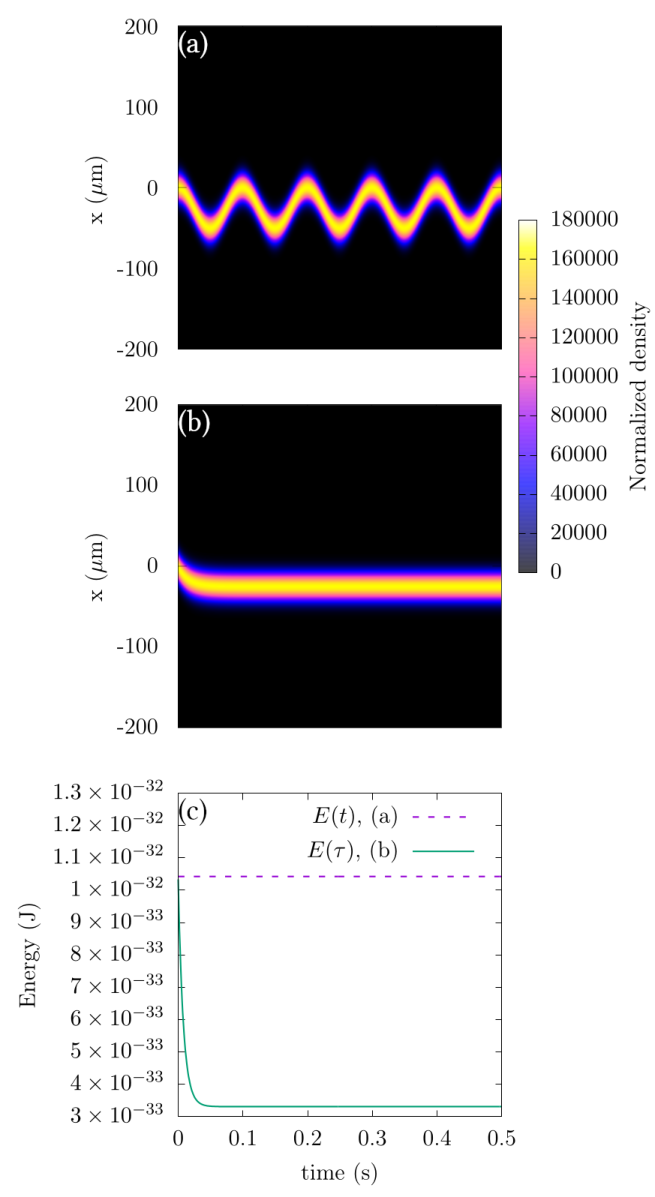
\includegraphics[width=0.6\textwidth]{data/splitop/SHO/SHO_gimp.pdf}

\caption{Evolution of a simple harmonic oscillator in (a) real, and (b) imaginary time after slightly shifting the trapping potential in the $\hat x$ direction.
In (c), we see the energy as a function of time and show that the energy of the system when evolving in real time remains constant, but in imaginary time it will decay to the known ground-state energy of the simple harmonic oscillator.
The simulated results are from evolution with the SSFM after 10,000 steps.
Here, we use a Rubidium 87 atom with $\omega_x = 10$Hz on a 256-point grid of size 200 $\mu$m, where the trap has been shifted by 5 $\mu m$.
The wavefunction has been normalized such that $\int_{-\infty}^\infty|\Psi|^2 dx = 1$.
This simulation was performed with the GPUE codebase \cite{schloss2018}.
\jrs{WIP}}
\label{fig:evolve}
\end{figure}

In addition to this, we can find the lowest energy state of our system with the SSFM by performing a Wick rotation and using $\tau = it$ for the simulation instead of traditional units of time~\cite{wick1954}.
This changes the solution from the complex sinusoid shown in Equation~\eqref{eqn:rsolve} to an exponential decay,

\begin{equation}
\Psi(\mathbf{r},\tau + d\tau) = \left[e^{-\frac{\mathcal{\hat{H}}d\tau}{\hbar}}\right]\Psi(\mathbf{r},\tau) = \sum_{n=0}^N\left[e^{-\frac{(E_n d\tau)}{\hbar}}\right]\Psi_n(\mathbf{r},\tau).
\end{equation}

\noindent This has two notable effects:
\begin{enumerate}
\item There will be an exponential decay of all higher-energy states, leaving only the ground state.
\item We see an exponential decay in the wavefunction density and therefore require renormalization regularly during the imaginary-time evolution.
\end{enumerate}
Let me start with a discussion on the first point, by showing a simulation of the same system as in Figure~\ref{fig:evolve}(a), but in imaginary time, shown in Figure~\ref{fig:evolve}(b).
Here, we see that the wavefunction density is shifting to the center of the trap, and
in Figure~\ref{fig:evolve}(c), we see the energy decaying to the known ground-state energy of a quantum harmonic oscillator of $\frac{1}{2}\hbar\omega = 3.31\times 10^{-33}$.
Here, the energy is computed as,
\begin{equation}
E = \braket{\Psi(\mathbf{r})|\hat H|\Psi(\mathbf{r})}
\label{eqn:energy}
\end{equation}
This is because all eigenstates of the wavefunction are affected by the exponential decay, with the ground state decaying the slowest, and because renormalization occurs every timestep, only the ground state will survive imaginary time propagation.

For many systems, we can assume the simulation is in the ground state when the energy converges to a fixed value.
More quantitatively, this means that the simulation can be completed when the change in energy every step in imaginary time is below some provided threshold; however, this is not always the best course-of-action.
Further discussion on energy calculations performed in this work will be shown in Chapter~\ref{ch:gpu}.

Now to discuss the second point, which is more problematic from a software perspective.
In practice, every step in imaginary time requires a relatively costly renormalization step with

\begin{equation}
    \label{eqn:norm}
    \int_\infty^\infty |\Psi(\mathbf{r},t)|^2 d\mathbf{r} = 1,
\end{equation}

\noindent for a single-particle wavefunction.
Computationally, this operation requires a summation, which is not well-optimized for GPU hardware; however, it is possible to perform a parallel reduction (summation), which allows for a considerable improvement on massively parallel systems~\cite{harris2007}.
Even so, the normalization is still a slow operation and should be used sparingly.

The implementation of the SSFM provided here assumes large-scale element-wise matrix multiplications in position and momentum-space; however, even though this implementation lends itself to parallelization, we will see other methods in Chapter~\ref{ch:gpu} when we discuss the implementation of the SSFM on graphics processing units.
Now we will turn our focus to systems to be simulated via the SSFM throughout this work: ultracold atoms.

\section{Introduction to ultracold quantum systems}
\label{sec:intro}

When atomic systems are cooled to temperatures near zero Kelvin, it becomes easier to discern their quantum properties which vary drastically depending on whether the particles are bosonic or fermionic.
Because fermions have half-integer spin, they must obey the Pauli exclusion principle and are constrained to Fermi--Dirac statistics at zero temperature.
This creates a \textit{Fermi sea}, where the particles fill defined energy levels from the bottom-up with two particles of opposite spin per level.
On the other hand, bosons have integer spin and follow Bose--Einstein statistics.
They will condense into a single, macroscopic ground state when cooled~\cite{einstein1925, fetter2003}, and
this state of matter is known as a Bose--Einstein Condensate (BEC).
The BEC has the properties of a superfluid, which will be discussed more completely in the following section.

There are notable exceptions to these rules, such as the highly correlated Tonks--Girardeau gas where bosons may act as spinless, non-interacting fermions \cite{girardeau1960, schloss2016}.
Though there also exists a regime where interacting fermions can condense into a BEC-like system by forming molecules with integer spin~\cite{nozieres1985, bulgac2014}, we will not discuss fermionic systems further in this work.
For now, we will focus on BEC systems, but will also discuss Tonks--Girardeau gas systems later in Chapter~\ref{ch:1d}.

\subsection{Bose--Einstein condensation and the Gross--Pitaevskii Equation}

For this section, we will follow a straightforward derivation using the second quantization~\cite{aversa2008}.
As mentioned in Section~\ref{sec:intro}, bosons in a BEC condense into a single ground state, meaning we must introduce a many-body Hamiltonian for the system and take inter-particle interactions into account.
Because experimental syustems are dilute, we will only consider two-body interactions and assume any interactions between three or more atoms to be unlikely and negligible.
We can write the Hamiltonian with two body interactions in the second quantized form as
\begin{equation}
    \mathcal{\hat H} = \int \hat \Psi^\dagger(\mathbf{r})\left[-\frac{\hbar^2}{2m}\nabla^2 + V_0(\mathbf{r}) \right]\hat \Psi(\mathbf{r}) d\mathbf{r} + \frac{1}{2} \int  \hat \Psi^\dagger(\mathbf{r}) \hat \Psi^\dagger(\mathbf{r'}) V(\mathbf{r} - \mathbf{r'})\hat \Psi(\mathbf{r'}) \hat \Psi(\mathbf{r}) d\mathbf{r} d\mathbf{r'}
    \label{eqn:2nd}
\end{equation}
where $\mathbf{r}$ and $\mathbf{r'}$ are the positions of the two colliding particles, $V(\mathbf{r}-\mathbf{r'})$ is the interaction potential, and $\hat \Psi^\dagger(\mathbf{r})$ and $\hat \Psi(\mathbf{r})$ are the creation and annihilation operators that follow the bosonic commutation relations,
\begin{align}
 [\hat \Psi(\mathbf{r}),\hat \Psi^\dagger(\mathbf{r})] &= \delta(\mathbf{r} - \mathbf{r'}) \\
 [\hat \Psi^\dagger(\mathbf{r}),\hat \Psi^\dagger(\mathbf{r})] &= 0 \\
 [\hat \Psi(\mathbf{r}),\hat \Psi(\mathbf{r})] &= 0.
\end{align}

\noindent In the case of a BEC at $T\approx0$, we may perform a Bogoliubov expansion~\cite{bogoliubov1947, dalfovo1999}
\begin{equation}
    \hat \Psi (\mathbf{r}, t) = \Phi(\mathbf{r},t) + \delta \hat \Phi(\mathbf{r},t),
\label{eqn:bog}
\end{equation}
where $\Phi(\mathbf{r},t) \equiv \langle \hat \Psi(\mathbf{r},t) \rangle$ is the wavefunction of the condensate known as the order parameter and $\delta \hat \Phi(\mathbf{r},t)$ represents fluctuations of the BEC system.
For Equation~\eqref{eqn:bog1} I have used the Heisenberg representation for field operators~\cite{dalfovo1999}.
In a BEC, the condensate density is defined as
\begin{equation}
    n(\mathbf{r},t) = |\Phi(\mathbf{r},t)|^2.
\end{equation}

Now we may use the Heisenberg equation of motion,
\begin{equation}
    i\hbar \frac{\partial}{\partial t}\hat \Psi(\mathbf{r},t) = [\hat \Psi, \hat H],
\end{equation}
    to determine the time evolution of the field operator $\hat \Psi(\mathbf{r},t)$ as
\begin{equation}
    \frac{\partial}{\partial t}\hat \Psi(\mathbf{r},t) = \frac{1}{i\hbar}\left[-\frac{\hbar^2}{2m}\nabla^2 + V_0(\mathbf{r}) + \int d\mathbf{r'} \hat \Psi^\dagger(\mathbf{r'}, t)V(\mathbf{r'} -\mathbf{r})\hat \Psi(\mathbf{r'},t)\right]\hat \Psi(\mathbf{r},t),
\end{equation}
which follows from Equation~\eqref{eqn:2nd} after integrating over $\mathbf{r}$.
If we assume that two bosons will only interact with a contact potential of the form
\begin{equation}
V(\mathbf{r'}-\mathbf{r}) = g\delta(\mathbf{r'} - \mathbf{r}),
\end{equation}
which has a strength given by
\begin{equation}
g \equiv \frac{4 \pi \hbar^2 a_s}{m},
\end{equation}
where $a_s$ is the species and state-dependent s-wave scattering length,
we may write the time-dependent Schr\"odinger equation as
\begin{equation}
    i\hbar \frac{\partial}{\partial t}\Phi(\mathbf{r},t) = \left( - \frac{\hbar^2}{2m} \nabla^2 + V_0(\mathbf{r}) + g |\Phi(\mathbf{r},t)|^2\right)\Phi(\mathbf{r},t).
\end{equation}

\noindent This is the Gross--Pitaevskii Equation (GPE), which is known as a governing equation for the physics of BEC systems.
When written in the time-independent form it determines the chemical potential $\mu$ of the condensate system~\cite{gross1961, pitaevskii1961}
\begin{equation}
    \mu\Phi(\mathbf{r}) = \left( - \frac{\hbar^2}{2m} \nabla^2 + V_0(\mathbf{r}) + g |\Phi(\mathbf{r})|^2\right)\Phi(\mathbf{r}).
    \label{eqn:GP}
\end{equation}

\noindent This equation allows us to determine the full dynamics of a BEC system and the numerical solutions will be discussed in subsequent chapters.
Similar derivations of the GPE can be found in many introductory texts on BEC physics~\cite{fetter2003, pethick2002, fetter2009}.
The main difference between this equation and the Schr\"odinger equation is the non-linear interaction term of $g|\Psi|^2$, that accounts for the fact that BECs typically consist of $10^3$ to $10^6$ particles..
When solving this system in a simple harmonic oscillator in the limit where interactions are significant, we will find a slightly different distribution for the wavefunction density, known as a Thomas--Fermi distribution, shown in Figure~\ref{fig:TF} for a single dimension.

The Thomas--Fermi distribution in this case can be derived from the time-independent GPE in the limit where there are a large number of bosons in the condensate ($N \gg 1$) as~\cite{ueda2010}
\begin{equation}
\Psi_\text{TF}(\mathbf{r}) = \sqrt{\frac{[\mu-V(\mathbf{r})\Theta(\mu-V(\mathbf{r})}{g}}
\end{equation}
\noindent where $\Theta$ is the Heaviside step function that ensures the condensate stays positive and $\Psi(\mathbf{r})_\text{TF}$ is the wavefunction in the Thomas--Fermi limit.
The shape of this function is similar to that of an inverted parabola for a harmonic trap, and the radius in any direction from the center can be found to be
\begin{equation}
R_\text{TF} = \sqrt{\frac{2\mu}{m\omega_i^2}}
\label{eqn:rtf}
\end{equation}
\noindent where $R_\text{TF}$ is the Thomas--Fermi radius and $\omega_i$ is the trapping frequency in the $i$th direction.
In the case of multiple particles, the normalization condition becomes $\int_{-\infty}^\infty |\Psi(\mathbf{r},t)|^2 = N$, where $N$ is the total number of particles.
By using this normalization condition, we find that the Thomas--Fermi chemical potential is
\begin{equation}
\mu_\text{TF} = \frac{h\omega_i}{2}\left(\frac{15 N a_s}{a} \right)^{2/5},
\label{eqn:mutf}
\end{equation}
\noindent where $a=\sqrt{\hbar/m\bar\omega}$ and $\bar omega$ is the average of all the harmonic trapping frequencies.
Using Equations~\eqref{eqn:mutf} and \eqref{eqn:rtf} we find that
\begin{equation}
R_\text{TF} = a\left(\frac{15 N a_s}{a} \right)^{1/5}\frac{\bar \omega}{\omega_i}
\end{equation}
This approximation is valid for stationary condensate solutions in simple harmonic oscillator trapping geometries.

\begin{figure}
\center 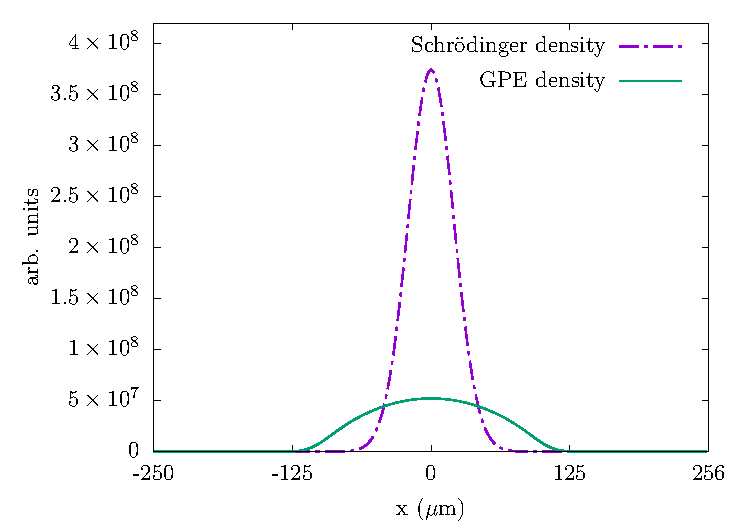
\includegraphics[width = \textwidth]{data/qs/SHO/SHO.pdf}

\caption{Ground state of simple harmonic oscillator for the Schr\"odinger equation (purple, dashed) and the GPE (cyan).
Here, we see that the GPE solution follows a Thomas-Fermi distribution, while the Schr\"odinger equation is Gaussian.
This simulation was performed with GPUE~\cite{schloss2018} for a two-dimensional grid of $256^2$ elements of size $250 \mu m$ with a trapping potential of $\omega_x = \omega_y = 1$, and $1\times 10^6$ particles.}
\label{fig:TF}
\end{figure}

It is important to note that a BEC acts like a superfluid, which is a state of matter that is similar to a classical fluid without viscosity.
This means that once a superfluid is set in motion, there is no retarding force to keep it from flowing.
There are a few known systems in which superfluidity can exist, such as $^4$He (sometimes called Helium II when in its superfluid phase)~\cite{allen1938}, neutron stars~\cite{migdal1960}, or BEC systems~\cite{einstein1925, anderson1995}.
BEC systems are generally cleaner experimental systems to create, as they do not have a classical fluid fraction, like $^4$He.
As stated, we will focus on BEC systems in this work, but it is important to note that any results shown in this body of work for BEC systems may have applications beyond cold, atomic physics.

\section{Superfluid systems and vortex dynamics}

Though there are many interesting differences between classical fluids and superfluids, such as sound wave propagation and turbulent dynamics, we will focus here on vortex dynamics before continuing to discuss three methods of vortex generation in superfluid systems: rotation, phase imprinting and artificial magnetic fields.
By rotating a fluid, it is possible to create a vortex around the axis of rotation; however, because of the viscosity of a classical fluid, the vortex will eventually disappear without constant driving.
In a superfluid, this is not necessarily the case.
To properly describe the differences in fluid and superfluid dynamics, it is worthwhile to discuss the hydrodynamic description of a BEC, following the text of Pethick and Smith~\cite{pethick2002},
To start, I will treat the condensate wavefunction as
\begin{equation}
\Psi(\mathbf{r},t) = \sqrt{\rho(\mathbf{r},t)}e^{i\phi(\mathbf{r},t)},
\label{eqn:ansatz}
\end{equation}
\noindent with
\begin{equation}
\rho(\mathbf{r},t)=\Psi(\mathbf{r},t)^*\Psi(\mathbf{r},t) = |\Psi(\mathbf{r},t)|^2.
\end{equation}
\noindent where $\phi(\mathbf{r},t)$ is the BEC phase.
By multiplying the GPE by $\Psi^*(\mathbf{r},t)$ and subtracting out the complex conjugate of the result, one can obtain the continuity equation~\cite{pethick2002},
\begin{equation}
\frac{\partial}{\partial t}\rho(\mathbf{r},t)+\nabla\cdot\mathbf{J}(\mathbf{r},t) = 0,
\end{equation}
\noindent where $\mathbf{j}$ is the current density of the condensate, defined as,
\begin{equation}
\mathbf{j}(\mathbf{r},t) = \frac{-i\hbar}{2m}\left( \Psi^*(\mathbf{r},t)\nabla\Psi(\mathbf{r},t)- \Psi(\mathbf{r},t)\nabla\Psi^*(\mathbf{r},t)\right).
\label{eqn:current_density}
\end{equation}
By substituting Equation~\eqref{eqn:ansatz} into Equation~\eqref{eqn:current_density}, we find the form of the current density for the GPE to be,
\begin{equation}
\mathbf{j}(\mathbf{r},t) = |\Psi(\mathbf{r},t)|^2\frac{\hbar}{m}\nabla\phi(\mathbf{r},t).
\end{equation}

The velocity of the superfluid is defined as a ratio of the current density to the density, itself, which is
\begin{equation}
\mathbf{v}(\mathbf{r},t)=\frac{\mathbf{j}(\mathbf{r},t)}{\rho(\mathbf{r},t)} = \frac{\hbar}{m}\nabla\phi(\mathbf{r},t).
\end{equation}
\noindent this can be interpreted to mean that the gradient of the phase determines the velocity of atoms in the BEC, indicating that the system is irrotational ($\nabla \times \mathbf{v} = 0$).
Because the condensate is single-valued, 
\begin{equation}
\oint \mathbf{v} \cdot d\ell = \frac{\hbar}{m}2\pi\ell.
\label{eqn:quantized}
\end{equation}
\noindent Here, $\ell$ is an integer charge of circulation, and Equation~\eqref{eqn:quantized} shows the quantized nature of circulation in a superfluid with each vortex hosting multiples of $2\pi$ charge.
Every singly-charged vortex in a BEC will have a $2\pi$ phase winding, and an example simulation with one vortex and its corresponding phase can be seen in Figure~\ref{fig:rot} (a and c).
Equation~\eqref{eqn:quantized} also indicates that the phase is not defined at the center of the vortes; however, at this point, the density has also dropped to zero.
The density dip from the normal condensate density to zero happens over the scale of the healing length.
For repulsive interactions, the healing length is
\begin{equation}
\xi=\frac{1}{\sqrt{8\pi\rho_ba_s}}
\end{equation}
\noindent where $\rho_b$ is the bulk density of the condensate.

\begin{figure}

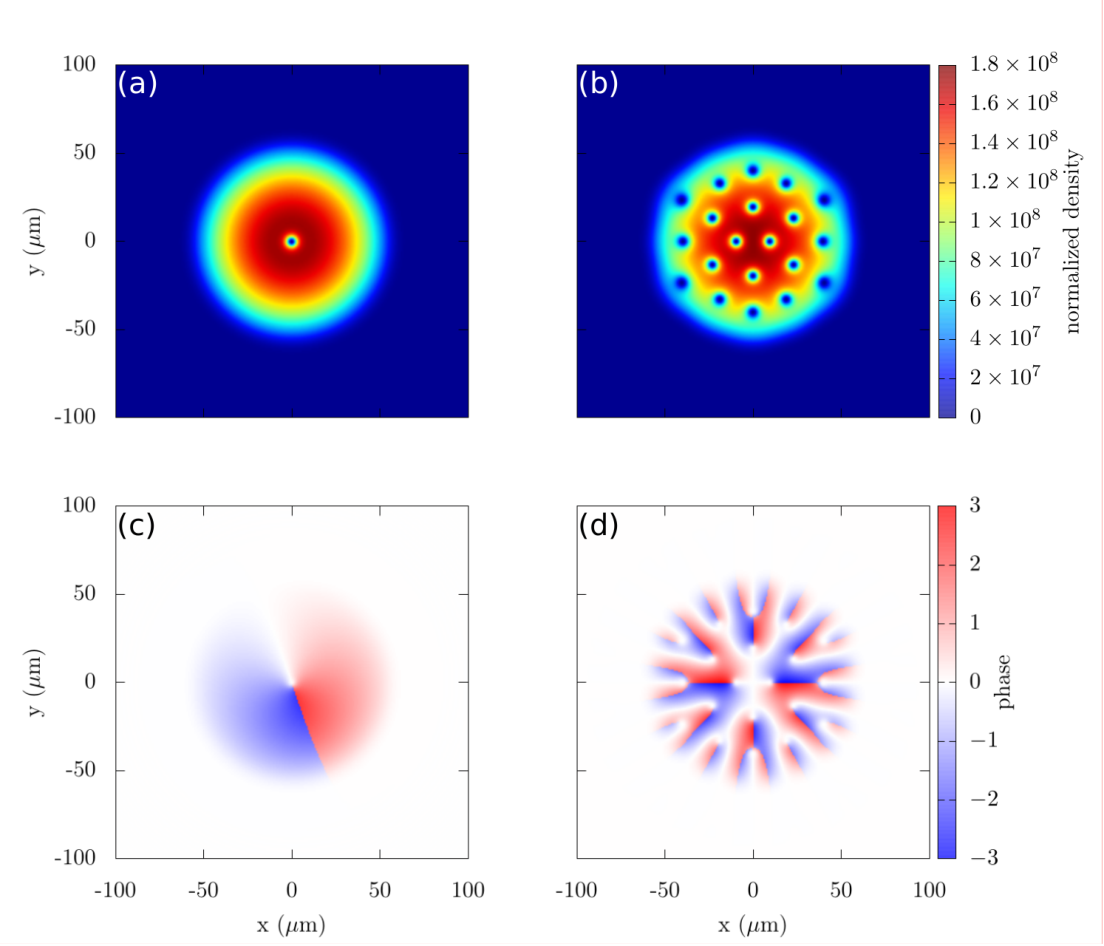
\includegraphics[width=\textwidth]{data/splitop/rot/WIP.pdf}

\caption{
Simulation of rotation with a single vortex (a, b) and a vortex lattice (c, d).
The wavefunction density is shown in a and c, while the corresponding phase is shown in b and d.
A rotation of $\Omega = 0.35\omega_x$ was used for a and b, while a rotation of $\Omega = 0.99\omega_x$ was used for c and d.
Here, we use a Rubidium 87 atom with $\omega_x = 2\pi$Hz on a 512-point grid of size 200 $\mu$m.
This simulation was performed with the GPUE codebase \cite{schloss2018}, and the phase plots are created by multiplying the phase by the wavefunction density to remove anomalous noise beyond the BEC boundary.
\jrs{WIP}}
\label{fig:rot}
\end{figure}

In a cyllindrically symmetric condensate with a single vortex at its center, the wavefunction can be written as
\begin{equation}
\Psi(\mathbf{r}) = |\Psi(\mathbf{r})|e^{i\ell\phi}
\end{equation}
And when substituting this in to Equation~\eqref{eqn:energy} for the GPE, we find
\begin{equation}
E = \int_{-\infty}^\infty \frac{\hbar^2}{2m}\left( |\nabla\Psi(\mathbf{r})|^2 + \frac{|\Psi(\mathbf{r})|^2\ell^2 m\mathbf{v}^2}{2}\right) + V_0(\mathbf{r})|\Psi(\mathbf{r})|^2 + \frac{g}{2}|\Psi(\mathbf{r})|^4.
\end{equation}
\noindent Because $E \propto \ell^2$\jrs{CN}, as a superfluid is spun faster beyond a critical angular velocity, a vortex will not grow or shrink in angular momentum, but multiple vortices will spawn instead~\cite{pethick2002}.
In other words, it is energetically favorable for two vortices of smaller angular momentum to form instead of a single vortex with a large amount of angular momentum.
As angular momentum increases and more vortices are introduced into the system, they will eventually arrange themselves in a triangular lattice structure known as an Abrikosov lattice~\cite{abrikosov1957, fetter2001}.
This behavior is identical to that of type II superconductors under the effects of a magnetic field, and the size of each vortex is described by a physical scale known as the healing length.
An example of a vortex lattice and its phase can be seen in Figure~\ref{fig:rot} (b and d).

The three-dimensional properties of vortices in superfluid systems are also peculiar when compared to their classical counterparts.
Here, vortex lines are formed that must either end at the end of the condensate~\cite{madison2000} or reconnect in the form of vortex rings or other, more complicated vortex structures~\cite{reichl2013, barenghi2014}.
Because the circulation around superfluid vortices is quantized, when two vortices approach each other with different velocity fields, they may reconnect into smaller, more energetically favorable vortex structures.
During this reconnection, the abrupt change in energy will create a sound wave at the reconnection site~\cite{feynman1955}.

Three dimensional vortex structures of non-trivial topology have been notoriously difficult to controllably generate experimentally, but we will discuss an experimentally viable method to generate, control, and detect vortex ring-like structures in superfluid BEC systems in Chapter~\ref{ch:vortex_states}.
In that chapter, I will also further discuss three-dimensional vortex motion.
 For now, we will begin discussing the three primary processes to generate vortex structures in superfluid systems: rotation, phase imprinting, and artificial magnetic fields.

\subsection{Rotation}

\label{sec:rot}
Rotation of a BEC system will provide vortex lines that follow the axis of rotation and start and end on the BEC boundary.
To simulate the effects of rotation, we simply need to append the angular momentum operator $L_z = -i\hbar(xp_y - yp_x)$ to the GPE,

\begin{equation}
i \hbar \frac{\partial \Psi(\mathbf{r},t)}{\partial t} = \left(\frac{p^2}{2m} + V_0 + g |\Psi(\mathbf{r},t)|^2 -\Omega L_z \right)\Psi(\mathbf{r},t),
\label{eqn:GPErot}
\end{equation}

\noindent where $\Omega$ is the rotation frequency. 

In order to generate a vortex via rotation in a harmonic trap, we must rotate faster than the critical velocity of $\Omega_c \approx 0.3 \omega_\perp$, where $\omega_\perp$ is the trapping frequency~\jrs{CN}.
In addition, if the rotation frequency is greater than the trapping frequency, the atoms will no longer be bound by the trap due to centripetal forces.
As such, finding the appropriate rotation frequency for creating vortex lattices in BEC systems is a precarious balancing act.
Even so, large scale vortex lattices have been generated both experimentally and theoretically, with the largest vortex lattices being generated with $\Omega \approx \omega_\perp$ \cite{o2016, o2016topo, abo2001, schweikhard2004}.

Experimentally, rotation is achieved by...

In this work, we use rotation in a qualitatively similar way to Equation~\eqref{eqn:GPErot}; however, we will later introduce artificial magnetic fields, which is a broader framework that encompass rotation and will be used in all our simulations moving forward.
We will discuss this in more detail in Section~\ref{sec:implementation}.

\subsection{Phase imprinting}

Phase imprinting is a powerful tool to allow for the generation of various structures in atomic systems, including vortices~\cite{kumar2018, moulder2012, burger1999, denschlag2000, wu2002}.
To generate vortices in a BEC, this technique relies on imprinting a $2\pi$ phase winding onto a ground state condensate wavefunction.
Experimentally, phase imprinting can be done in a number of ways.
As an example, the phase could be imprinted with a Raman two-photon process to transfer orbital angular momentum to atoms from a Laguerre--Gaussian beam \cite{moulder2012, ryu2007}.
Another method is through pulsing a spatially dependent potential for a short time when compared to the trapping frequency, which will imprint the potential energy onto the phase of the system~\cite{kasevich1991} and can be used to generate solitons~\cite{denschlag2000}, vortex~\cite{gajda1999}, or other states with quantized circulation~\cite{kumar2018}.
Phase imprinting has also been used in theoretical studies to create a defect in a large vortex lattice by flipping the phase (and therefore rotation direction) of a selected vortex by imprinting a $-4\pi$ phase at the vortex's location~\cite{o2016topo}.
Note that if a phase greater than $|2\pi|$ is imprinted onto the system, the vortices are likely to decay into multiple vortices of $|2\pi|$ phase~\cite{shin2004}.

For the purposes of this work, we will only consider imprinting vortex lines along the transverse plane by apply phase imprinting operations to our condensate, such that

\begin{equation}
\Psi_{\text{IMP}}(x,y,t) = |\Psi(x,y,t)|e^{i(\theta(x,y,t) + \theta_{\text{IMP}}(x,y))},
\end{equation}

\noindent where $\Psi_{\text{IMP}}(x,y,t)$ is the condensate wavefunction after phase imprinting.
This method allows us to apply a phase mask to any location in the transverse plane.
This technique will be applied further in Chapter~\ref{ch:2d}.

Phase imprinting has allowed for the generation of many interesting vortex topologies in theoretical and experimental studies~\cite{white2014, maucher2016}; however, it is a dynamical process that does not create eigenstates of the system.
As such, it is not as useful for engineering stable vortex structures, but is instead useful for dynamical studies, such as those found in Chapter~\ref{ch:2d}.

\subsection{Artificial magnetic fields}
\label{sec:gauge}

Magnetic fields are capable of generating rotational effects in charged systems through the Lorentz force, $F_l = q(\mathbf{E} + \mathbf{v} \times \mathbf{B})$, where $q$ is the charge of the system, $\mathbf{E}$ is the electric field, $\mathbf{B}$ is the magnetic field, and $\mathbf{v}$ is the velocity of the particle.
This effect allows for the creation of vortices in type II superconductors; however, it is not directly applicable to BEC systems, because BECs are composed of neutral atoms.
Even so, it is possible to generate artificial magnetic fields with similar effects, and these artificial magnetic fields have  been shown to create vortices experimentally~\cite{lin2009}.
In addition, artificial magnetic fields create a broader framework that encompasses rotational effects previously shown in Section~\ref{sec:rot}, and we will use this framework instead of rotation for remainder of this work.
As such, a detailed introduction, similar to that given by Dalibard in~\cite{dalibard2015}, will be presented below.

If written in the Hamiltonian formalism, the Lorentz force law becomes

\begin{equation}
\mathcal{\hat{H}} = \frac{(\mathbf{\hat p} - q\mathbf{A}(\mathbf{r}))^2}{2m}
\end{equation}

\noindent where $\mathbf{A}$ is a vector potential such that $\mathbf{B} = \nabla \times \mathbf{A}$ and $q$ is the charge of the particle.
Because cold atoms are neutral, we must find ways to simulate the effects of magnetic fields instead of using magnetic fields, themselves.

Firstly, let us describe how rotation can be considered to be an artificial vector potential and thus generate vortex structures in BEC systems.
Imagine a plane rotating with an angular velocity $\Omega$ around the $z$-axis ($\mathbf{\Omega} = \Omega \hat z$). 
In this case, the Coriolis force is defined as
\begin{equation}
\mathbf{F}_{\text{Coriolis}} = 2m \mathbf{v} \times \mathbf{\Omega},
\end{equation}
which is formally similar to the Lorentz force law.
By applying the transformation $\mathcal{\hat H} = \hat H_0 - \Omega \hat L_z$, where $\hat L_z = x\partial_y - y\partial_x$, we find~\cite{bhat2008}
\begin{equation}
\begin{split}
\mathcal{\hat H} &= -\frac{\hbar^2}{2m}\nabla^2 + \frac 1 2 m \omega^2(x^2 + y^2) - \frac{\hbar \Omega}{i}(x\partial_y - y\partial_x) \\
 &= \frac{1}{2m}\left(\frac{\hbar}{i}\nabla - m(\mathbf{\Omega} \times \mathbf{r})\right)^2 + \frac m 2 \left( \omega^2 - \Omega^2 \right)r^2 \\
 &= \frac{(\hat{\mathbf{p}}-m\mathbf{A}(\mathbf{r}))^2}{2m}+ V_0(\mathbf{r}),
\end{split}
\end{equation}
where $\omega$ is the trapping frequency for a symmetric two-dimensional harmonic trap, $\mathbf{A} \equiv \mathbf{\Omega} \times \mathbf{r}$, and $V_0 = m/2 \left( \omega^2 - \Omega^2 \right)r^2$.
The final form is similar to that of the Lorentz force law and coincides with an effective magnetic field of $2 \mathbf \Omega \propto \mathbf B$.
In this way, we may recreate the rotation expected from the Lorentz force law in a cold atomic system with an artificial magnetic field~\cite{peshkin1989, madison2000, abo2001}.

Artificial magnetic fields provide a powerful tool to researchers who wish to generate and control complex vortex structures, and because of this, it is worth discussing them in further detail.
Important implementation details for how to use artificial magnetic fields with the SSFM will be discussed in Section~\ref{sec:implementation}.

\subsubsection{Geometric Gauge Fields}
\label{sec:geom}

As we have already described how rotation can act as an artificial Lorentz force, we now turn our attention towards methods that might allow us to generate more general rotational effects and vortex structures.
In particular, we will discuss the adiabatic motion of free atoms undergoing geometric phase transformations through the Berry phase. 
For this, we assume that our system has an external parameter $\lambda$ such that
\begin{equation}
\hat H(\lambda) \ket{\psi_n(\lambda)} = E_n(\lambda)\ket{\psi_n(\lambda)},
\end{equation}
where the set of eigenstates $\left\{ \ket{\psi_n(\lambda)} \right\}$ allows us to define the time evolution of our system such that
\begin{equation}
\ket{\psi(t)} = \sum_n c_n(t) \ket{\psi_n(\lambda(t))},
\end{equation}
and we consider $\lambda$ to evolve slowly with time. If we consider the system to begin with
\begin{equation}
c_l(0) = 1,
\qquad
c_n(0) = 0, 
\qquad
\text{for all } n\neq l
\end{equation}
the state of the system is proportional to $\ket{\psi_l(\lambda(t))}$.
In this case, $c_l(t)$ is determined by the equation
\begin{equation}
i \hbar \dot{c}_l =  [E_l(t) - \dot{\lambda} \cdot \mathbf{A}_l(\lambda)]c_l,
\label{Bcnx-1}
\end{equation}
where 
\begin{equation}
\mathbf{A}_l(\lambda) = i \hbar \braket{\psi_l|\nabla\psi_l}.
\label{eqn:Bcnx}
\end{equation}
This quantity is called the Berry connection, which is considered a vector potential, such that we can define a new artificial magnetic field, the Berry curvature as
\begin{equation}
\mathbf{B}_l = \mathbf{\nabla} \times \mathbf{A}_l.
\label{eqn:BC}
\end{equation}

Now imagine that the $\lambda$ parameter follows the closed contour $C$ such that $\lambda(T) = \lambda(0)$. 
By integrating Equation~\eqref{Bcnx-1} above, we find
\begin{equation}
c_l(t) = e^{i \Phi_{\text{dyn}}(t)}e^{i\Phi_{\text B}(T)}c_l(0),
\label{eqn:c}
\end{equation}
where
\begin{equation}
\begin{split}
\Phi_{\text{dyn}}(T) &= - \frac{1}{\hbar}\int_0^TE_l(t)dt \\
\Phi_{\text{Berry}} (T)&= \frac{1}{\hbar} \int_0 ^T \dot{\lambda} \cdot \mathbf{A}_l(\lambda)dt = \frac{1}{\hbar}\oint\mathbf{A}_l(\lambda) \cdot d\lambda
\end{split}
\end{equation}
In this case $\Phi_{\text{Berry}}$ is called the Berry phase and it only depends on the motion path of $\lambda$. 
It should be mentioned that both of the exponential terms in Equation~\eqref{eqn:c} are gauge invariant and thus remain unchanged when $\ket{\psi_n(\lambda)}$ is multiplied by a phase factor.
This phase allows us to transfer angular momentum into our BEC and generate a vortex geometry like those formed in the 2009 experiment by Lin~\textit{et~al.}~\cite{lin2009}.
As a note, the vortex structures generated in this way follow the magnetic fields lines, thus providing the capability to generate complex vortex structures beyond vortex lines.
Outside of rotation, another method to generate these gauge fields in an experimentally realizable way with the evanesent field of a dielectric system undergoing total internal reflection will be described in Chapter~\ref{ch:vortex_states}, but for now we should discuss how these fields can be implemented in the SSFM, with an emphasis on their effects for superfluid simulations.

\section{Modifications to the SSFM for superfluid vortex simulations}
\label{sec:implementation}

As shown above, in order to simulate the effects of artificial magnetic fields on BEC systems, we must slightly modify the Hamiltonian, such that

\begin{equation}
\mathcal{\hat H} = \frac{(p-m\mathbf{A})^2}{2m} + V_0 + g|\Psi(\mathbf{r},t)|^2,
\end{equation}

\noindent where $\mathbf{A}$ is an artificial vector potential.
As a note, some texts absorb the mass term into the artificial vector potential, but here we are stating it explicitly for clarity.
When expanded, we note that the gauge field has a component in position space, $\frac{m\mathbf{A}^2}{2}$, which couples with the trapping potential, and another component that is partially in both position and momentum space, $p\mathbf{A}$.

Firstly, let us discuss the component purely in position space.
Here, we see that it is important to properly balance the trapping potential and the artificial vector potential when simulating BEC systems with artificial vector potentials, otherwise, the trapping geometry will become warped.
In the case of rotation, this is effectively balanced by the centripetal force; however, 
in the case of arbitrarily chosen vector potentials, this can create rather unusual potential geometries, as shown in Figure~\ref{fig:V_change} for a Gaussian $\mathbf{A_x}$ and $\mathbf{A_y}$.
Though we might be able to balance this warping with a centripetal force tailored to the gauge fields we introduce, we did not consider this for the purposes of this work.

\begin{figure}

\center 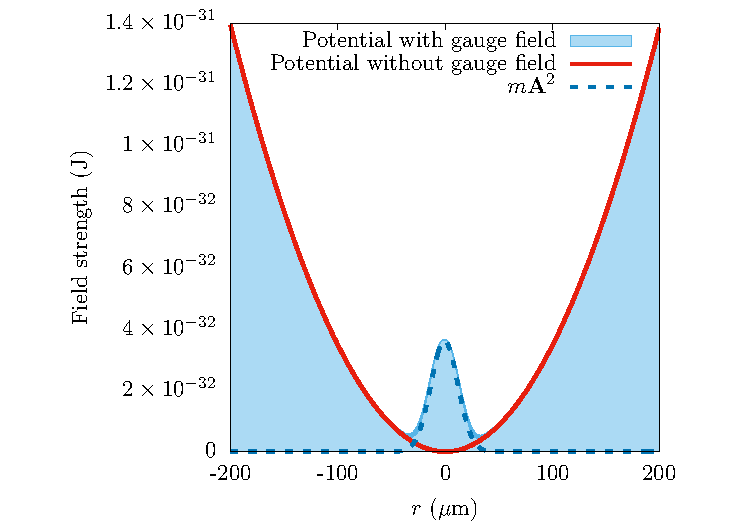
\includegraphics[width=0.6\textwidth]{data/splitop/gauge/check.pdf}

\caption{
Simulation of GPE with an arbitrarily chosen Gaussian artificial vector potential.
For this simulation, we have removed the $pA$ term to focus on the warped potential, itself.}
\label{fig:V_change}
\end{figure}

The components of the artificial vector potential that are partially in position and momentum space are somewhat difficult to consider numerically.
As they reside in both spaces, it is required to perform a one-dimensional FFT across $n$-dimensional data.
This means that if we have three operators, $p\mathbf{A}_x \hat x$, $p\mathbf{A}_y \hat y$, and $p\mathbf{A}_z \hat z$, we will need to perform an FFT on our wavefunction in the $\hat x$, $\hat y$, and $\hat z$ dimensions, respectively, before applying the operators through element-wise multiplication. 
As I will discuss in Chapter~\ref{ch:gpu}, this has significant performance penalties if we do not consider the massively parallel GPU architecture.
This also requires the usage of more intricate FFT plans for the FFTW or CuFFT libraries, which are non-trivial for three-dimensional simulations.

\section{Multi-component simulations}

Until now, the discussion has been oriented around single-component condensates; however, in recent years, there has been a significant amount of theoretical and experimental interest in multiple BEC components in the same system~\jrs{CN}.
When simulating such systems, the GPE must be modified to take interactions between components into account and each wavefunction must be evolved separately, such that 

\begin{equation}
i \hbar \frac{\partial \Psi_i(\mathbf{r},t)}{\partial t} = \left(\frac{(p-mA)^2}{2m} + V_0 + \sum_{j=1}^C g_{ij}|\Psi_j(\mathbf{r},t)|^2 \right)\Psi_i(\mathbf{r},t)
\label{eqn:GPE}
\end{equation}

\noindent where $C$ is the total number of components being simulated, $\Psi_i(\mathbf{r},t)$ for $i \in {0,...,C}$ is the wavefunction for a unique component being evolved, and $g_{ij}$ is the interaction strength between components $i$ and $j$.
The interaction matrix is symmetric, such that $g_{ji} = g_{ij}$, and there are generally three mixing regimes in which multi-component condensates can be found:

\begin{description}
\item[No interaction] In this regime, $g_{ij}=0$, while $g_{ii} = 1$. This creates an interaction matrix that is identical to the identity matrix and can be understood as a simulation of $C$ GPE components without interaction. It is rare that these simulations will be performed, simply because the additional components will produce identical results unless the atomic species is modified, and there is no reason to perform a non-interacting multi-component simulation rather than multiple single-component simulations.
\item[Miscible] In this regime, $0 < g_{ij} < 1$ and the $C$ components mix in some fashion. This means that there will be some differentiation between components, but they can still exist in the same physical space.
\item[Immiscible] In this regime, $g_{ij} \geq 1$ and the $C$ components no longer mix and therefore cannot exist in the same physical locations as other components.
\end{description}

ADD FIGURE

In Figure~\ref{fig:multicomp}, I show simulations for a three component condensate in each of these three regimes for a rotating system.
These simulations are memory-intensive, but we will discuss several methods to minimize the memory footprint of single-component simulations in Chapter~\ref{ch:gpu}.
These methods also apply to multicomponent simulations and allow for simulations with a higher component number.

At this point, we have discussed the SSFM, itself, along with the primary system we will be simulating in this work; however, we have yet to discuss key techniques in quantum engineering that are necessary to motivate several design decisions.
As such, we will consider two dynamic methods for quantum state engineering in the following chapter: shortcuts to adiabaticity and quantum optimal control.

